% ============================================================
%  Lecture 4 — Routing and packing problems
%  (still Chapter 1: Introduction to Scheduling)
% ============================================================

\section{Routing Problems}
\label{sec:routing}

The last family of problems in our survey comes from
\textbf{logistics}: given a set of locations to visit and
distances between them, find the cheapest way to serve everyone.%
\aside{TSP and VRP are among the most studied
problems in combinatorial optimisation.}

% ------------------------------------------------------------
\subsection{The Travelling Salesman Problem (TSP)}
\label{ssec:tsp}
% ------------------------------------------------------------

\begin{definition}[Travelling Salesman Problem]
\label{def:tsp}
Given a complete, undirected, edge-weighted graph
$G = (V, E, c)$ with $n$ nodes and edge costs $c_{ij} \ge 0$,
find a \emph{Hamiltonian cycle} (a cycle that visits every node
exactly once) of minimum total cost.
\end{definition}

In plain words: a salesperson must visit every city and return
home, travelling the shortest possible route.%
\aside{A non-complete graph can be made complete
by adding shortest-path edges.}

The number of distinct Hamiltonian cycles on $n$ nodes is
$(n-1)!/2$, which grows faster than any exponential.
TSP is $\NP$-hard; there is no known polynomial-time exact
algorithm.

\paragraph{Greedy 1: Nearest Neighbour.}
Start at a \emph{depot} node.
At each step, move to the \emph{closest unvisited} node.
After all nodes are visited, return to the depot.

\begin{example}[Nearest Neighbour]
\label{ex:nn-tsp}
On a small graph with 8 nodes, suppose the nearest-neighbour
tour starting from node~1 follows
$1 \to 2 \to 3 \to 8 \to 4 \to 5 \to 6 \to 7 \to 1$
with total cost~24.  The algorithm is fast---$\Oh{n^2}$---but
can make globally poor choices: a city left until last may
force a long detour back.
\end{example}

\begin{remark}
Any tour with \emph{crossing edges} is provably suboptimal:
the crossing can always be ``uncrossed'' to reduce the cost.
Nearest Neighbour frequently produces crossings, which is a
visual sign that the solution can be improved.
\end{remark}

\paragraph{Greedy 2: Insertion.}
Start with a small subtour (e.g.\ the depot plus one node).
At each step, choose an unvisited node and a position in the
current tour, and \emph{insert} the node where it increases the
tour cost the least.
Variants differ in how the next node is chosen:
\begin{itemize}[nosep]
  \item \emph{Nearest insertion}: pick the unvisited node closest
        to the current tour.
  \item \emph{Farthest insertion}: pick the farthest---this
        often outperforms nearest insertion because it builds the
        ``skeleton'' of the tour early.
  \item \emph{Cheapest insertion}: pick the (node, position) pair
        that causes the smallest cost increase.
\end{itemize}
Insertion heuristics run in $\Oh{n^2}$ to $\Oh{n^3}$ depending on
the variant, and tend to produce fewer crossings than Nearest
Neighbour.


% ------------------------------------------------------------
\subsection{Vehicle Routing Problem (VRP)}
\label{ssec:vrp}
% ------------------------------------------------------------

\begin{definition}[Capacitated Vehicle Routing Problem---CVRP]
\label{def:cvrp}
Given:
\begin{itemize}[nosep]
  \item a complete, edge-weighted graph with a distinguished
        \emph{depot} node;
  \item $n$ \emph{customers}, each with a demand $q_i > 0$;
  \item a fleet of $K$ identical vehicles, each with
        capacity~$Q$.
\end{itemize}
Find a set of $K$ routes (cycles starting and ending at the
depot) such that:
\begin{enumerate}[nosep]
  \item every customer is visited by exactly one route;
  \item the total demand on each route does not exceed~$Q$;
  \item the total travel cost is minimised.
\end{enumerate}
\end{definition}

The CVRP generalises the TSP: with $K = 1$ and $Q = \infty$
it reduces to a TSP\@.  The extra dimension---splitting customers
across vehicles while respecting capacity---makes the problem
significantly harder.

\paragraph{Greedy approaches for VRP.}
All VRP heuristics come in \emph{sequential} (build one route at
a time) and \emph{parallel} (build all routes simultaneously)
flavours.

\subparagraph{Nearest Neighbour (sequential).}
Build one route: start at the depot, repeatedly visit the nearest
unvisited customer whose demand fits the remaining capacity.
When no more customers fit, return to the depot and start a new
route.  Risk: the last vehicle inherits far-flung customers.

\subparagraph{Nearest Neighbour (parallel).}
Start all vehicles at the depot.  At each step, extend the
vehicle whose nearest reachable customer is closest.
This avoids the ``last vehicle gets the leftovers'' problem.

\subparagraph{Clarke \& Wright Savings.}
\begin{enumerate}[nosep]
  \item Start with $n$ trivial routes: depot $\to$ customer $i$
        $\to$ depot, one per customer.
  \item For every pair of routes, compute the \emph{saving}
        $s_{ij} = c_{0i} + c_{0j} - c_{ij}$:
        the cost saved by merging the two routes instead of
        making two separate round-trips.
  \item Greedily merge the pair with the largest saving,
        provided the merged route respects capacity.
        Repeat until no more feasible merges improve cost.
\end{enumerate}

\subparagraph{Clustering + TSP.}
\begin{enumerate}[nosep]
  \item Partition customers into $K$ clusters (e.g.\ by
        geographic proximity), respecting vehicle capacity.
  \item Solve a separate TSP within each cluster.
\end{enumerate}
A variant: instead of explicit clustering, identify $K$
\emph{pivot} nodes (the farthest-apart customers), assign each
vehicle to a pivot, and run Nearest Neighbour from there.


% ------------------------------------------------------------
\subsection{VRP variants}
\label{ssec:vrp-variants}
% ------------------------------------------------------------

The CVRP is the simplest member of a large family.  Common
extensions include:

\begin{itemize}
  \item \textbf{Time windows (CVRPTW).}
    Each customer has a time interval $[e_i, l_i]$: the vehicle
    may arrive early (and wait), but not late.
    Waiting time becomes part of the route cost.

  \item \textbf{Heterogeneous fleet.}
    Vehicles differ in capacity, cost per km, or customer
    compatibility (e.g.\ some trucks cannot reach certain
    locations).

  \item \textbf{Multi-depot.}
    Several depots; each vehicle departs from (and may return to)
    any depot.

  \item \textbf{Prizes / Orienteering.}
    Not all customers must be visited.  Each customer offers a
    \emph{prize}; the objective balances travel cost against
    collected prizes.  With one vehicle this is the
    \emph{orienteering problem}; with several, the
    \emph{team orienteering problem}.

  \item \textbf{Pickup and delivery.}
    Some customers supply goods, others receive them.  Capacity
    must be checked at every point along the route, making the
    problem significantly harder.

  \item \textbf{Time-dependent costs.}
    Travel times depend on the time of day (rush hour, traffic).
    Routes become asymmetric: the cost of an edge depends on
    when it is traversed.

  \item \textbf{Electric vehicles.}
    Limited range; the vehicle must visit recharge stations.
    Route planning must account for battery state.

  \item \textbf{Vehicles and drones.}
    A truck carries a drone that can make short deliveries from
    the truck's current position, saving the truck from
    detours.

  \item \textbf{Refrigerated vehicles.}
    Energy cost for refrigeration depends on ambient temperature,
    which varies along the route and over time.
\end{itemize}


% ============================================================
\section{Bin Packing}
\label{sec:bin-packing}
% ============================================================

Bin packing generalises the knapsack: instead of one container,
we have as many as we need, and the goal is to use \emph{as few
as possible}.%
\aside{Knapsack: what fits in one bin?
Bin packing: how many bins for everything?}

% ------------------------------------------------------------
\subsection{1D Bin Packing}
\label{ssec:bin-packing-1d}
% ------------------------------------------------------------

\begin{definition}[1D Bin Packing]
\label{def:bin-packing-1d}
Given $n$ items with sizes $w_1, \dots, w_n$ and bins of
capacity~$W$, assign every item to a bin so that the total size
in each bin does not exceed~$W$ and the number of bins used is
minimised.
\end{definition}

\begin{example}[Six items, capacity 50]
\label{ex:bin-packing-6}
Items: $30, 4, 7, 12, 6, 40$.  Capacity $W = 50$.

\begin{figure}[H]
\centering
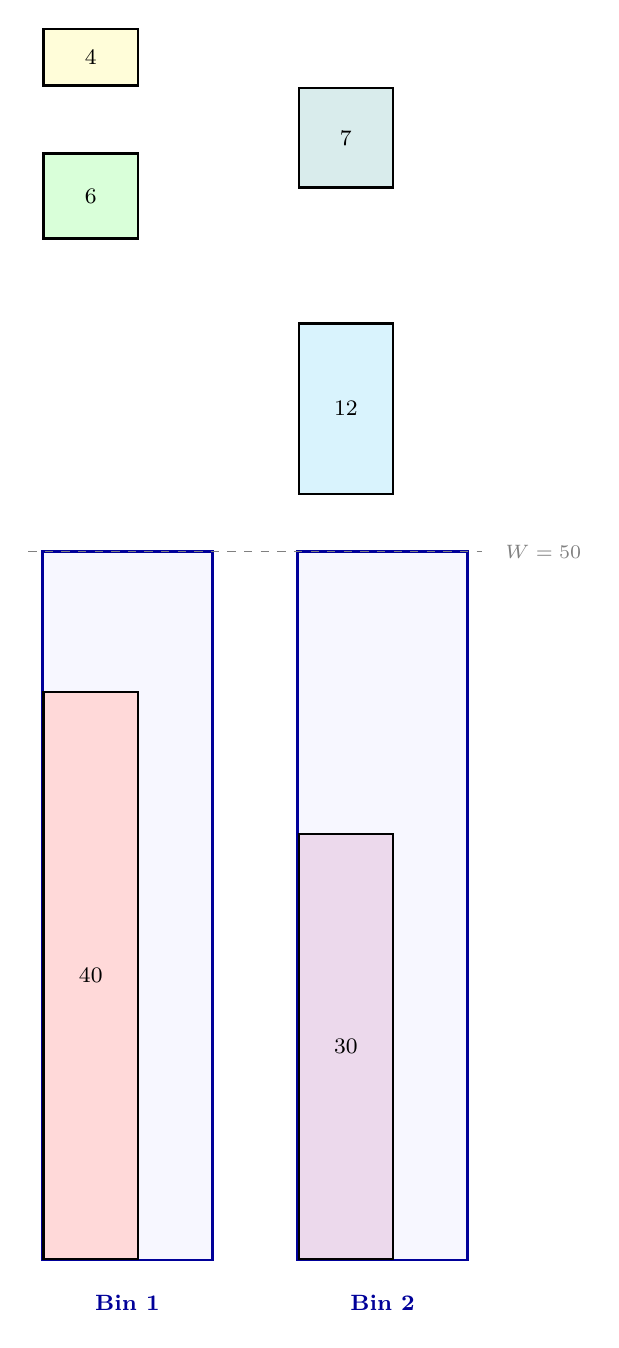
\begin{tikzpicture}[
    x=1.8mm, y=1.8mm,
    bin/.style={draw=blue!60!black, thick, fill=blue!3},
    item/.style={draw, thick, fill=orange!20,
                 font=\footnotesize, anchor=south west},
  ]
  % Bin 1
  \draw[bin] (0,0) rectangle (12, 50);
  \node[font=\footnotesize\bfseries, blue!60!black] at (6, -3) {Bin 1};
  \node[item, fill=red!15,    minimum width=12mm, minimum height=40*1.8mm] at (0, 0) {40};
  \node[item, fill=green!15,  minimum width=12mm, minimum height=6*1.8mm]  at (0, 72) {6};
  \node[item, fill=yellow!15, minimum width=12mm, minimum height=4*1.8mm]  at (0, 82.8) {4};

  % Bin 2
  \draw[bin] (18,0) rectangle (30, 50);
  \node[font=\footnotesize\bfseries, blue!60!black] at (24, -3) {Bin 2};
  \node[item, fill=violet!15, minimum width=12mm, minimum height=30*1.8mm] at (18, 0) {30};
  \node[item, fill=cyan!15,   minimum width=12mm, minimum height=12*1.8mm] at (18, 54) {12};
  \node[item, fill=teal!15,   minimum width=12mm, minimum height=7*1.8mm]  at (18, 75.6) {7};

  % capacity labels
  \draw[gray, dashed] (-1, 50) -- (31, 50);
  \node[font=\scriptsize, gray, anchor=west] at (32, 50) {$W = 50$};
\end{tikzpicture}
\caption{Optimal packing of six items into two bins (capacity 50).
         Bin~1: $40 + 6 + 4 = 50$.  Bin~2: $30 + 12 + 7 = 49$.}
\label{fig:bin-packing-optimal}
\end{figure}
\end{example}

\paragraph{Greedy heuristics for 1D Bin Packing.}

\subparagraph{First Fit (FF).}
Process items in the given order.  Place each item in the
\emph{first} bin where it fits; if none, open a new bin.

\subparagraph{Best Fit (BF).}
Process items in the given order.  Place each item in the bin
that will have the \emph{least remaining capacity} after
insertion (tightest fit); if none, open a new bin.

\subparagraph{First Fit Decreasing (FFD) / Best Fit Decreasing
  (BFD).}
Sort items by \emph{decreasing} size, then apply FF or BF\@.
Sorting large items first is a simple but effective improvement:
large items are the hardest to fit, so placing them early avoids
situations where a large item forces an extra bin at the end.

\begin{example}[Comparing heuristics on \cref{ex:bin-packing-6}]
\label{ex:bin-packing-greedy}
With items in the original order $30, 4, 7, 12, 6, 40$:
\begin{itemize}[nosep]
  \item \textbf{First Fit}: Bin~1 = $\{30, 4, 7, 6\}$ (47),
        Bin~2 = $\{12\}$ (12),
        Bin~3 = $\{40\}$ (40).
        \textbf{3 bins}.
  \item \textbf{Best Fit}: Bin~1 = $\{40, 7\}$ (47),
        Bin~2 = $\{30, 12, 6\}$ (48),
        Bin~3 = $\{4\}$ (4).
        \textbf{3 bins}.
\end{itemize}
With items sorted decreasingly ($40, 30, 12, 7, 6, 4$):
\begin{itemize}[nosep]
  \item \textbf{Best Fit Decreasing}: Bin~1 = $\{40, 7\}$ (47),
        Bin~2 = $\{30, 12, 6, \mathbf{?}\}$---12 + 30 = 42,
        then 6 fits (48), then 4 fits \emph{only in Bin~1}
        (47 + 4 > 50, so new bin).
        Actually: Bin~1 = $\{40, 7\}$, Bin~2 = $\{30, 12, 6\}$,
        Bin~3 = $\{4\}$.  Still \textbf{3 bins}---but on many
        instances BFD significantly outperforms FF\@.
\end{itemize}
The optimum (2 bins) requires a more global view:
Bin~1 = $\{40, 6, 4\}$ (50), Bin~2 = $\{30, 12, 7\}$ (49).
\end{example}

% ------------------------------------------------------------
\subsection{2D and 3D Bin Packing}
\label{ssec:bin-packing-2d3d}
% ------------------------------------------------------------

In higher dimensions, items and bins become geometric objects:

\paragraph{2D Bin Packing.}
Items are \emph{rectangles}; bins are larger rectangles.
Beyond deciding \emph{which} bin, we must decide \emph{where}
in the bin to place each item (coordinates) and possibly whether
to \emph{rotate} it 90\textdegree.

Placement heuristics typically maintain a list of ``corner
points''---positions where a new item can be placed flush against
existing items or bin walls---and choose the corner that wastes
the least space.

\begin{itemize}[nosep]
  \item \textbf{Strip packing}: pack items into horizontal
        strips; each strip is as tall as its tallest item.
        Simple but wastes vertical space.
  \item \textbf{Shelf algorithms}: a refinement of strip
        packing with rules for starting new shelves.
\end{itemize}

\noindent
Applications: cutting glass, wood, or sheet metal; VLSI layout;
page layout.

\begin{remark}[Guillotine cuts]
In glass and wood cutting, every cut must go \emph{edge to edge}
(a ``guillotine cut'').
This rules out L-shaped residual pieces: after cutting, both
resulting pieces must be rectangles.
The constraint significantly restricts the set of feasible
packings and requires specialised algorithms.
\end{remark}

\paragraph{3D Bin Packing / Container Loading.}
Items are \emph{boxes} (rectangular parallelepipeds); bins are
shipping containers.  Additional real-world constraints include:
\begin{itemize}[nosep]
  \item \textbf{Stability}: items must rest on a flat surface;
        no floating items.
  \item \textbf{Fragility}: heavy items cannot be stacked on
        fragile ones.
  \item \textbf{Weight balance}: the centre of gravity must stay
        within tolerance (especially for trucks and aircraft).
  \item \textbf{Rotation restrictions}: some items may only rest
        on certain faces (e.g.\ ``this side up'').
  \item \textbf{Loading order}: items needed first at delivery
        must be accessible (loaded last, near the door).
\end{itemize}

\begin{intermezzo}{From theory to practice}
The gap between textbook bin packing and industrial applications
is large.  A real glass-cutting optimiser must handle guillotine
constraints, material defects, different glass types, and client
grouping (pieces for the same order should come from the same
sheet to simplify logistics).  A container-loading solver must
model gravity, fragility, and access order.  The greedy
heuristics we have seen---First Fit, Best Fit, and their
decreasing variants---serve as building blocks inside these
richer systems, often as the constructive phase of a
metaheuristic.
\end{intermezzo}
